%% This is file `elsarticle-template-1-num.tex',
%%
%% Copyright 2009 Elsevier Ltd
%%
%% This file is part of the 'Elsarticle Bundle'.
%% ---------------------------------------------
%%
%% It may be distributed under the conditions of the LaTeX Project Public
%% License, either version 1.2 of this license or (at your option) any
%% later version.  The latest version of this license is in
%%    http://www.latex-project.org/lppl.txt
%% and version 1.2 or later is part of all distributions of LaTeX
%% version 1999/12/01 or later.
%%
%% Template article for Elsevier's document class `elsarticle'
%% with numbered style bibliographic references
%%
%% $Id: elsarticle-template-1-num.tex 149 2009-10-08 05:01:15Z rishi $
%% $URL: http://lenova.river-valley.com/svn/elsbst/trunk/elsarticle-template-1-num.tex $
%%
\documentclass[preprint,12pt]{elsarticle}

%% Use the option review to obtain double line spacing
%% \documentclass[preprint,review,12pt]{elsarticle}

%% Use the options 1p,twocolumn; 3p; 3p,twocolumn; 5p; or 5p,twocolumn
%% for a journal layout:
%% \documentclass[final,1p,times]{elsarticle}
%% \documentclass[final,1p,times,twocolumn]{elsarticle}
%% \documentclass[final,3p,times]{elsarticle}
%% \documentclass[final,3p,times,twocolumn]{elsarticle}
%% \documentclass[final,5p,times]{elsarticle}
%% \documentclass[final,5p,times,twocolumn]{elsarticle}

%% The graphicx package provides the includegraphics command.
\usepackage{graphicx}
%% The amssymb package provides various useful mathematical symbols
\usepackage{amssymb}
%% The amsthm package provides extended theorem environments
%% \usepackage{amsthm}

%% The lineno packages adds line numbers. Start line numbering with
%% \begin{linenumbers}, end it with \end{linenumbers}. Or switch it on
%% for the whole article with \linenumbers after \end{frontmatter}.
\usepackage{lineno}

%% natbib.sty is loaded by default. However, natbib options can be
%% provided with \biboptions{...} command. Following options are
%% valid:

%%   round  -  round parentheses are used (default)
%%   square -  square brackets are used   [option]
%%   curly  -  curly braces are used      {option}
%%   angle  -  angle brackets are used    <option>
%%   semicolon  -  multiple citations separated by semi-colon
%%   colon  - same as semicolon, an earlier confusion
%%   comma  -  separated by comma
%%   numbers-  selects numerical citations
%%   super  -  numerical citations as superscripts
%%   sort   -  sorts multiple citations according to order in ref. list
%%   sort&compress   -  like sort, but also compresses numerical citations
%%   compress - compresses without sorting
%%
%% \biboptions{comma,round}

% \biboptions{}

\journal{Journal Name}

\begin{document}

\begin{frontmatter}

%% Title, authors and addresses

\title{Unnecessarily Complicated Research Title}

%% use the tnoteref command within \title for footnotes;
%% use the tnotetext command for the associated footnote;
%% use the fnref command within \author or \address for footnotes;
%% use the fntext command for the associated footnote;
%% use the corref command within \author for corresponding author footnotes;
%% use the cortext command for the associated footnote;
%% use the ead command for the email address,
%% and the form \ead[url] for the home page:
%%
%% \title{Title\tnoteref{label1}}
%% \tnotetext[label1]{}
%% \author{Name\corref{cor1}\fnref{label2}}
%% \ead{email address}
%% \ead[url]{home page}
%% \fntext[label2]{}
%% \cortext[cor1]{}
%% \address{Address\fnref{label3}}
%% \fntext[label3]{}


%% use optional labels to link authors explicitly to addresses:
%% \author[label1,label2]{<author name>}
%% \address[label1]{<address>}
%% \address[label2]{<address>}

\author{John Smith}

\address{California, United States}

\begin{abstract}
%% Text of abstract

\end{abstract}

\begin{keyword}
Science \sep Publication \sep Complicated
%% keywords here, in the form: keyword \sep keyword

%% MSC codes here, in the form: \MSC code \sep code
%% or \MSC[2008] code \sep code (2000 is the default)

\end{keyword}

\end{frontmatter}

%%
%% Start line numbering here if you want
%%
\linenumbers

%% main text
\section{Introduction}
\label{S:1}

\begin{itemize}
\item Risk and uncertainty
\item One rule for all?
\item Impact of life histories
\item Comparision of constant catch v changing catch based on trends in an empirical index. 
\end{itemize}

Sustainability and risks to non target exploited marine fish stock populations requires both estimates of current stock status, the effects of fishing pressure (catchability and fishing effort) and the effects of management measures on target populations, however these data are often lacking.  Subsequently there is increasing concern and a growing need for the development of innovative approaches so that management of all marine stocks not just those of high commercial value can be included into the Common Fisheries Policy (CFP \cite{EU 2013}) framework. Under the CFP management objectives are to recover stocks and to maintain stocks within safe biological limits to levels that can produce Maximum Sustainable Yield (MSY), including by-catch species by 2015 (Implementation Plan adopted at the World Summit on Sustainable Development, Johannesburg in 2002) and no later than 2020. These conservation objectives are currently being achieved by introducing biological target reference points e.g. population size (stock biomass) and/or yields (catches) and/or long–term yields and fishing mortality against which the preservation of stocks within such limits are assessed. These targets or reference points are often referred to as harvesting strategies which include an operational component called a harvest control rule (HCR) that are based on indicators (e.g. monitoring data or models) of stock status. 

The International Council for the exploration of the Sea (ICES) categorises stocks in to classes "data-rich", (categories 1 and 2) i.e those that have a quantitive assessment based on conventional mehods that require large amounts of data that include a long historical time series of catches and sound biological information \cite{Bentley, 2015}; or "data-limted" \cite{Costello et al 2015}(categories 3 and 4) (often called data poor) those without and assessment and forecasts. For data-rich stocks ICES uses two types of reference points for providing fisheries advice; 

1. Precautionary Approach (PA) reference points (those relating to stock status and exploitation relative to precautionary objectives) and 
2. MSY reference points (those relating to achieving MSY), 

In contrast for data limited stocks MSY 'proxy' reference points are used to estimate stock status and exploitation.  Often many of the methods used to estimate MSY proxy reference points require length based inputs as they are cheap, easy to collect \cite{Quinn and Deriso, 1999} and are related to life history paramters such as fish size, mortality and fecundity as well as fishery selectivity. For example many methods are being developed to estimate MSY, but currently only 4 are approved by ICES, these include, Surplus Production model in Continuous Time (catch based) (SPiCT; \cite{Pedersen and Berg, 2016}, Mean Length Z (MLZ; \cite{Gedamke & Hoenig, 2016}), Length Based Spawner Per Recruit (LBSPR; \cite{Hordyk et al 2015}) and Length Based Indicators (LBI; e.g. \cite{Probst et al 2013}). The aforementoned data limited procedures have differing data requirements, intended uses and obviously have their own strengths and weaknesses. 

To test the performance of candidate management procedures often requires evaluation of alternative hypothesis about the dynamics of the system e.g. population dynamics and the behaviour of the fishery (e.g life history dynamics, range contraction and density dependence) etc.. Due to the nature of conflicting objectives, stakeholder interests and the uncertainty in the dynamics of the resource and/ or the plausibility of alternative hypotheses can lead to poor decision making and can be problematic when defining management policy.

An intense area of work being researched over the last 2 decades is Management Strategy Evaluation (MSE), which focuses on the broader aspects of fishing (the Ecosystem) whereby different management options are tested against a range of objectives (see \cite{Kell et al., 2007}.  The approach is not to come up with a definitive answer, but to lay-bare the trade offs associated with each management objective, along with identifying and incorporating uncertainties in the evaluation and communicating the results effectively to client groups and decision-makers. MSE is not intended to be complex but to provide a robust framework that account for conflicting poorly defined objectives and uncertainties that have been absent in conventional management \cite{Kell et al., 2007}.  

To better understand the performance of a range of management procedures we aim to test generic empirical HCR (based on catch per unit effort – CPUE indices) that maximises yield without stock collapse for  a selection of ICES data-limited fisheries. Often empirical harvest control rules require extensive exhaustive parameter searches to tune hyper-parameters that aren’t directly learnt from estimators.  This requires a technique known as a grid search that extensively searches for all combinations of all parameters. In contrast and some what less time consuming, other efficient parameter search strategy’s can be considered for a given range of parameter space and a known distribution a sample can be obtained, and is known as a random search.  

To test case specific harvest strategies (via simulation) within the MSE, we will implement a management procedure based on a empirical harvest control rule that adjusts yield depending on stock status for a constant catch and a given range of hype-parameters for each empircal harvest strategy, and test their robustness to risk and uncertainty.  This approach could also help identify similar conditions across species where particular advice rules are likely to work well, and where they perform poorly for a given a set of hyper-parameters. Assessment will be made as to the performance of each HCR via a set of utilities: safety (a proportion, recruitment/virgin recruitment), yield (a proportion, $yield/MSY$), kobe proportion (proportion of years that stay in the green zone of kobe plot ($B/B_{MSY} >1$ and $F)/F_{MSY} < 1$, and Yield Annual Variation (yield changes by 10\% year on year). 

EU (2013) Regulation (EU) No 1380/2013 of the European Parliament and of the Council of 11 December 2013 on the Common Fisheries Policy, amending Council Regula- tions (EC) No 1954/2003 and (EC) No 1224/2009 and repealing Council Regulations (EC) No 2371/2002 and (EC) No 639/2004 and Council Decision 2004/585/EC. Off J Eur Union L 354:22−61
Bentley, N. 2015. Data and time poverty in fisheries estimation: potential approaches and solutions. ICES J. Mar. Sci. 72: 186–193.
Costello, C., Ovando, D., Hilborn, R., Gaines, S.D., Deschenes, O., and Lester, S.E. 2015. Status and solutions for the world’s unassessed fisheries. Science. 338: 517–20. doi: 10.1126/science.1223389.
Gedamke, T. and Hoenig, J.M. 2006. Estimating mortality from mean length data in nonequilibrium situations, with application to the assessment of goosefish. Transactions of the American Fisheries Society 135:476-487.
Hordyk, A.R., Ono, K., Sainsbury, K.J., Loneragan, N., and Prince, J.D. 2015b. Some explorations of the life history ratios to describe length composition, spawning-per- recruit, and the spawning potential ratio. ICES J. Mar. Sci. 72: 204–216.
Pedersen MW, Berg CW (2016) A stochastic surplus production model in continuous time. Fish Fish 18:226–243.
Probst, W. N., Kloppmann, M., and Kraus, G. 2013. Indicator-based status assessment of commercial fish species in the North Sea according to the EU Marine Strategy Framework Directive (MSFD). ICES Journal of Marine Science, 70: 694–706.
Quinn T. J., Deriso R. B., Quantitative Fish Dynamics, 1999. New YorkOxford University Press.

\section{Material and Methods}
\subsection{Materials}

Fishnets

\subsection{Methods}

FLife and MSE

\subsubsection{Operating Model}

Age based.

\subsubsection{Management Procedure}

The management procedure was based on an empirical MP, where an increase in an index of abundance resulted in an increase in the TAC, while a decrease in the index results in an decrease in the TAC.

\subsubsection{Random Search}

%https://stats.stackexchange.com/questions/160479/practical-hyperparameter-optimization-random-vs-grid-search

When running an MSE commonly a set of MP scenarios are run to tune the MP, this requires running the MSE for each OM scenario for a range of fixed values in the HCR and then choosing the rule that best meets management objectives. If there are a lot of parameters to tune then a grid search may become unfeasible. An alternative is random search \cite{bergstra2012random} as randomly chosen trials are more efficient for parameter optimisation than trials based on a grid. 

%For example any distribution over a sample space with a finite maximum, the maximum of 60 random observations lies within the top 5\% of the true maximum, with 95\% probability.  Imagine the 5\% interval around the true maximum. Now imagine that we sample points from his space and see if any of it lands within that maximum. Each random draw has a 5\% chance of landing in that interval, if we draw n points independently, then the probability that all of them miss the desired interval is (1−0.05)n So the probability that at least one of them succeeds in hitting the interval is 1 minus that quantity. We want at least a .95 probability of success. To figure out the number of draws we need, just solve for n in the equation: 1−(1−0.05)^n>0.95 We get n⩾60
  
\section{Results}

\textbf{[EXAMPLES TO BE UPDATED]}
\begin{itemize}
\item Figure \ref{fig:lh} shows the life history parameters
\item Figure \ref{fig:vector} shows the vectors
\item Figure \ref{fig:ts} shows the time series relative to reference points
\item Figure \ref{fig:pm} shows the performance statistics; points are
\begin{enumerate}
 \item ~
 \item ~
 \item ~
 \item ~\item Figure \ref{fig:util} shows the utility functions for the seven study stocks points area
\end{enumerate}
\begin{enumerate}
 \item ~
 \item ~
 \item ~
 \item ~
\end{enumerate}

\end{itemize}

\section{Discussion}


\begin{itemize}
\item Bullet point one
\item Bullet point two
\end{itemize}

\section{Conclusions}

\begin{itemize}
\item Bullet point one
\item Bullet point two
\end{itemize}

\section{References}

\bibliographystyle{model1-num-names}
\bibliography{/home/laurence/Desktop/flr/equations/tex/refs.bib} 

\section{Figures}

\begin{figure}[]\centering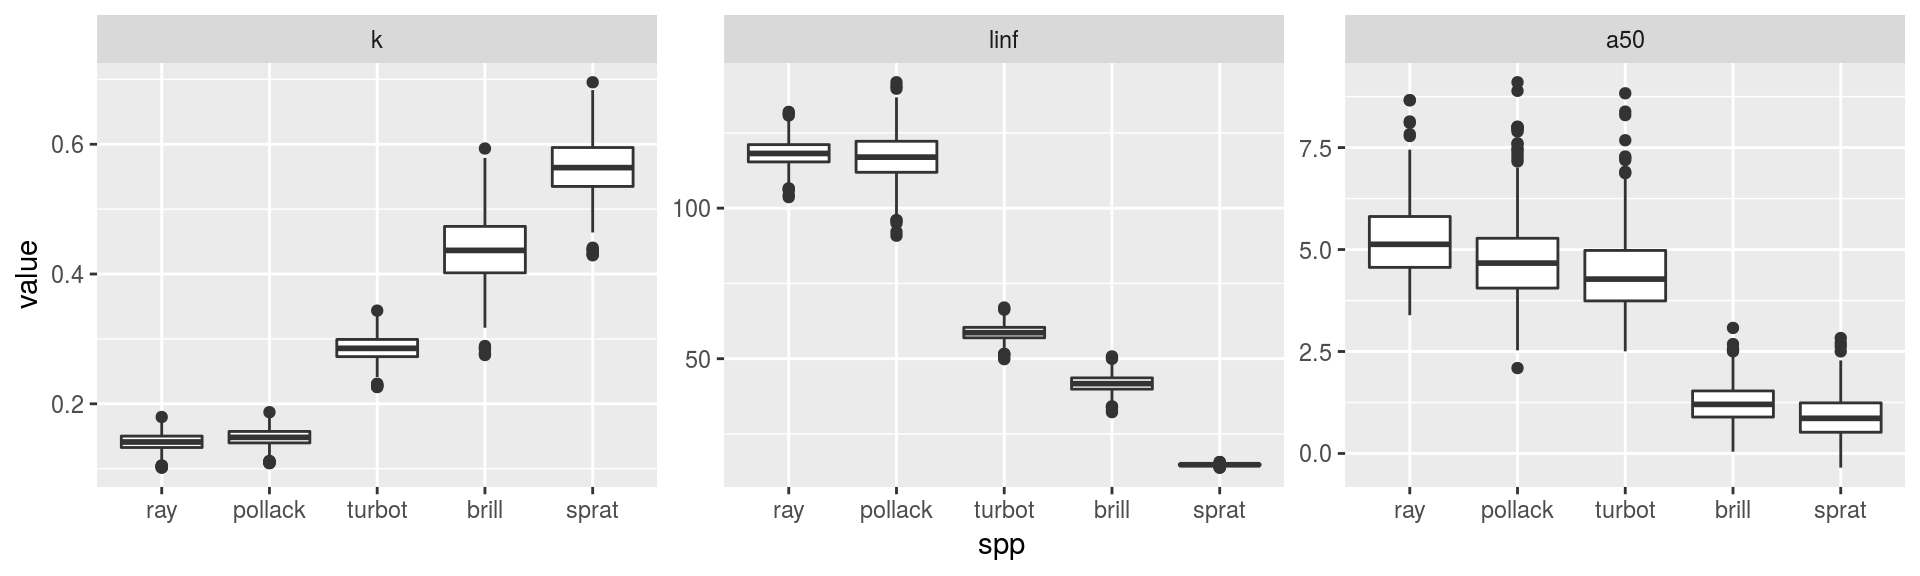
\includegraphics[width=5in]{rg-lhpar-1.png}\caption{}\label{fig:lh}\end{figure}
\begin{figure}[]\centering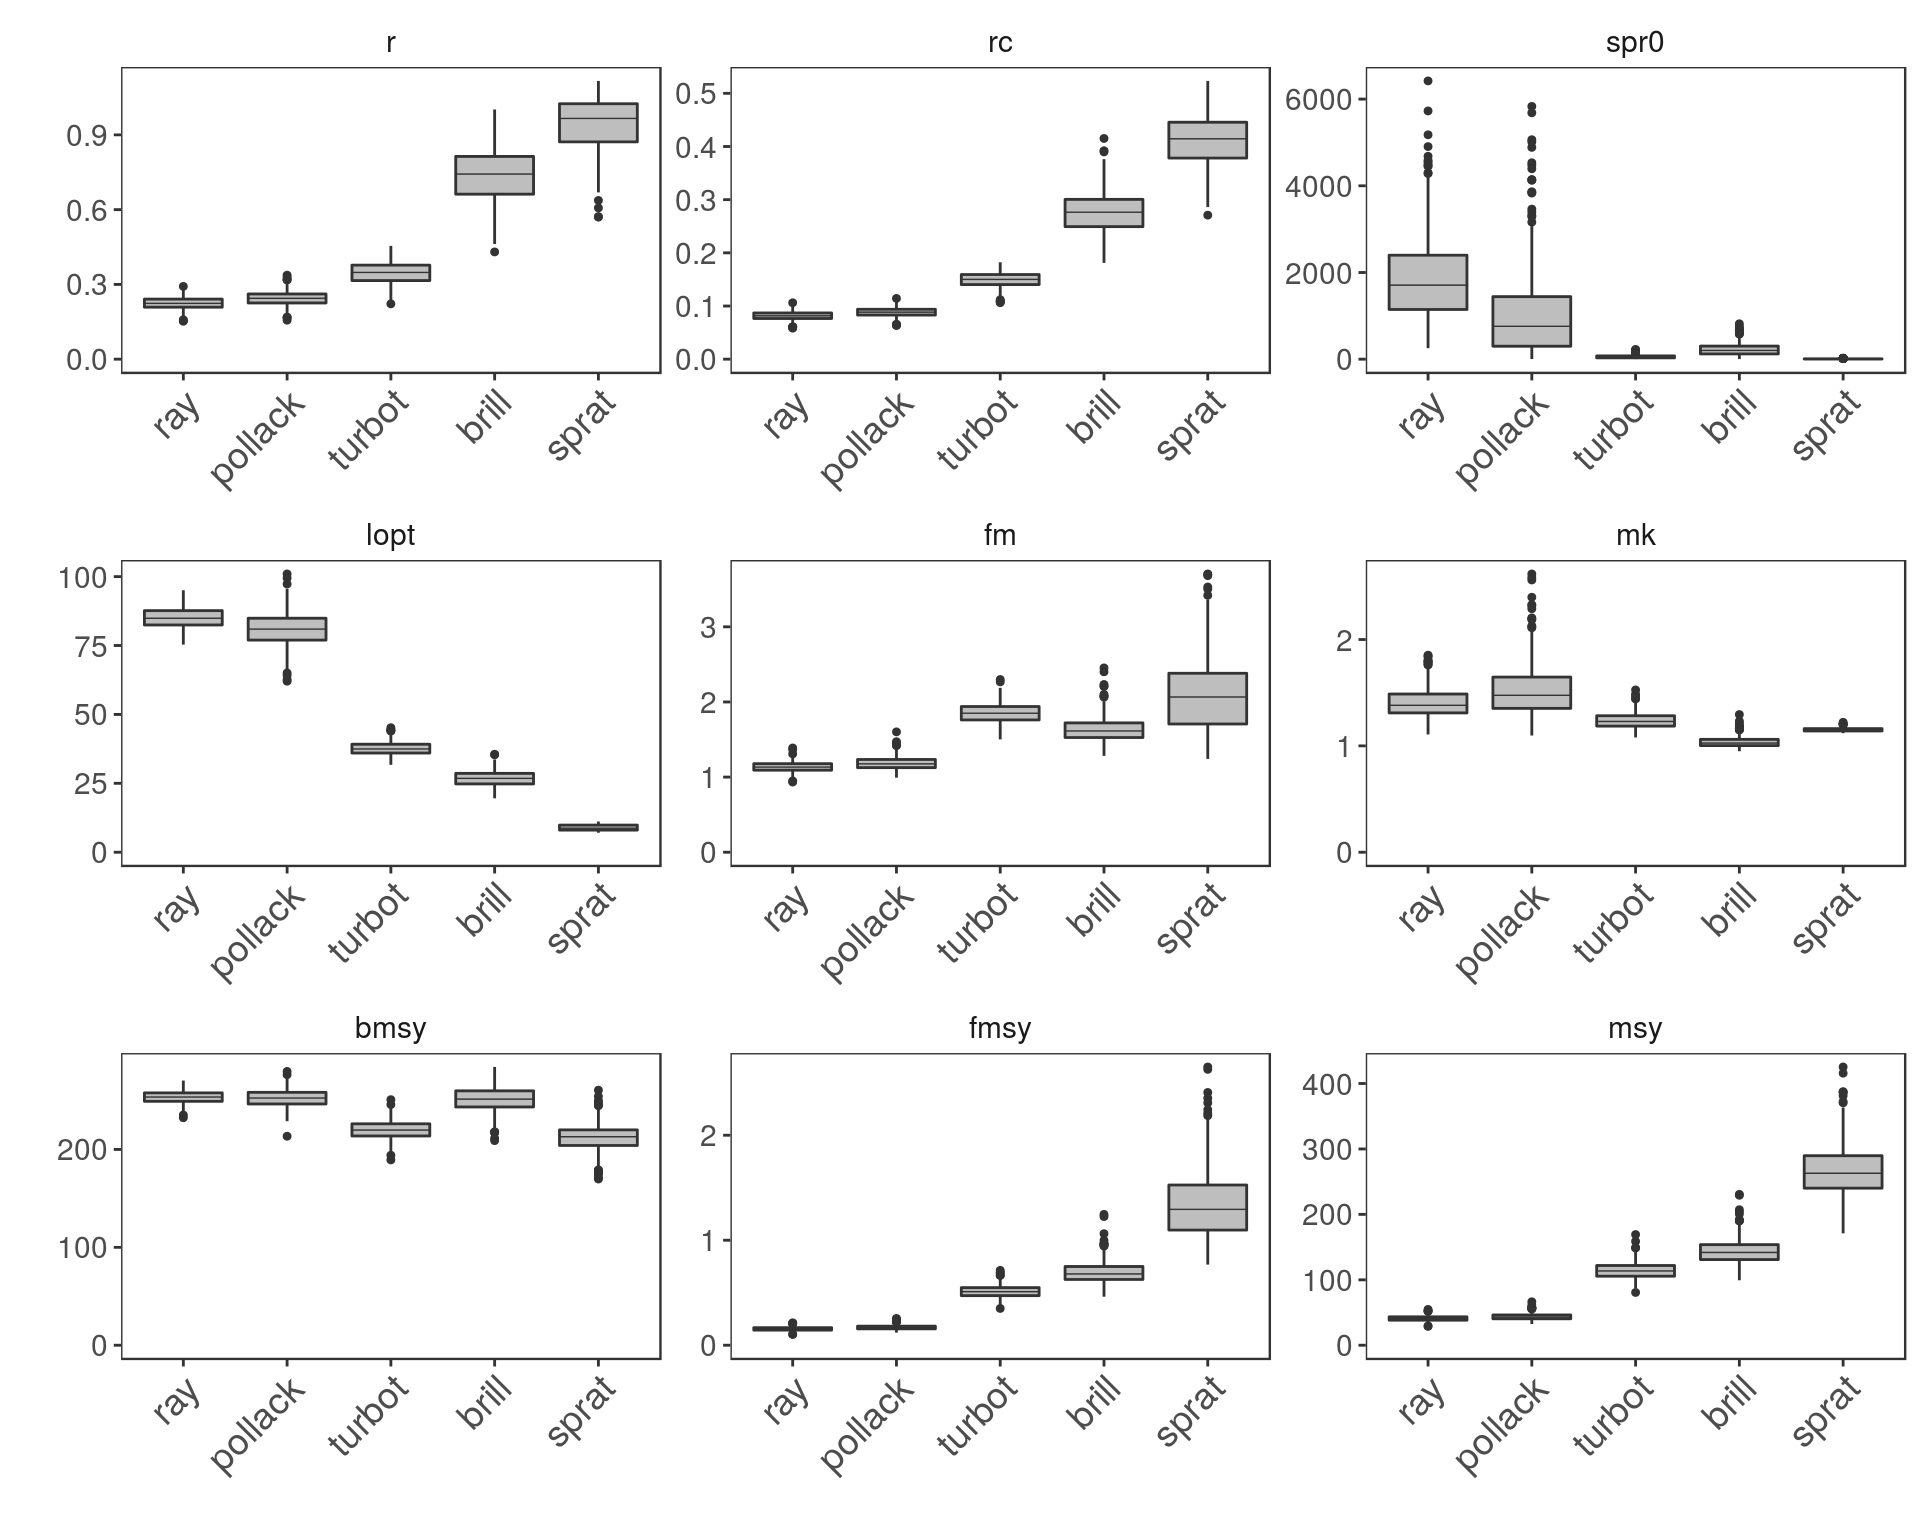
\includegraphics[width=5in]{rg-derived-1.png}\caption{}\label{fig:lh}\end{figure}
\begin{figure}[]\centering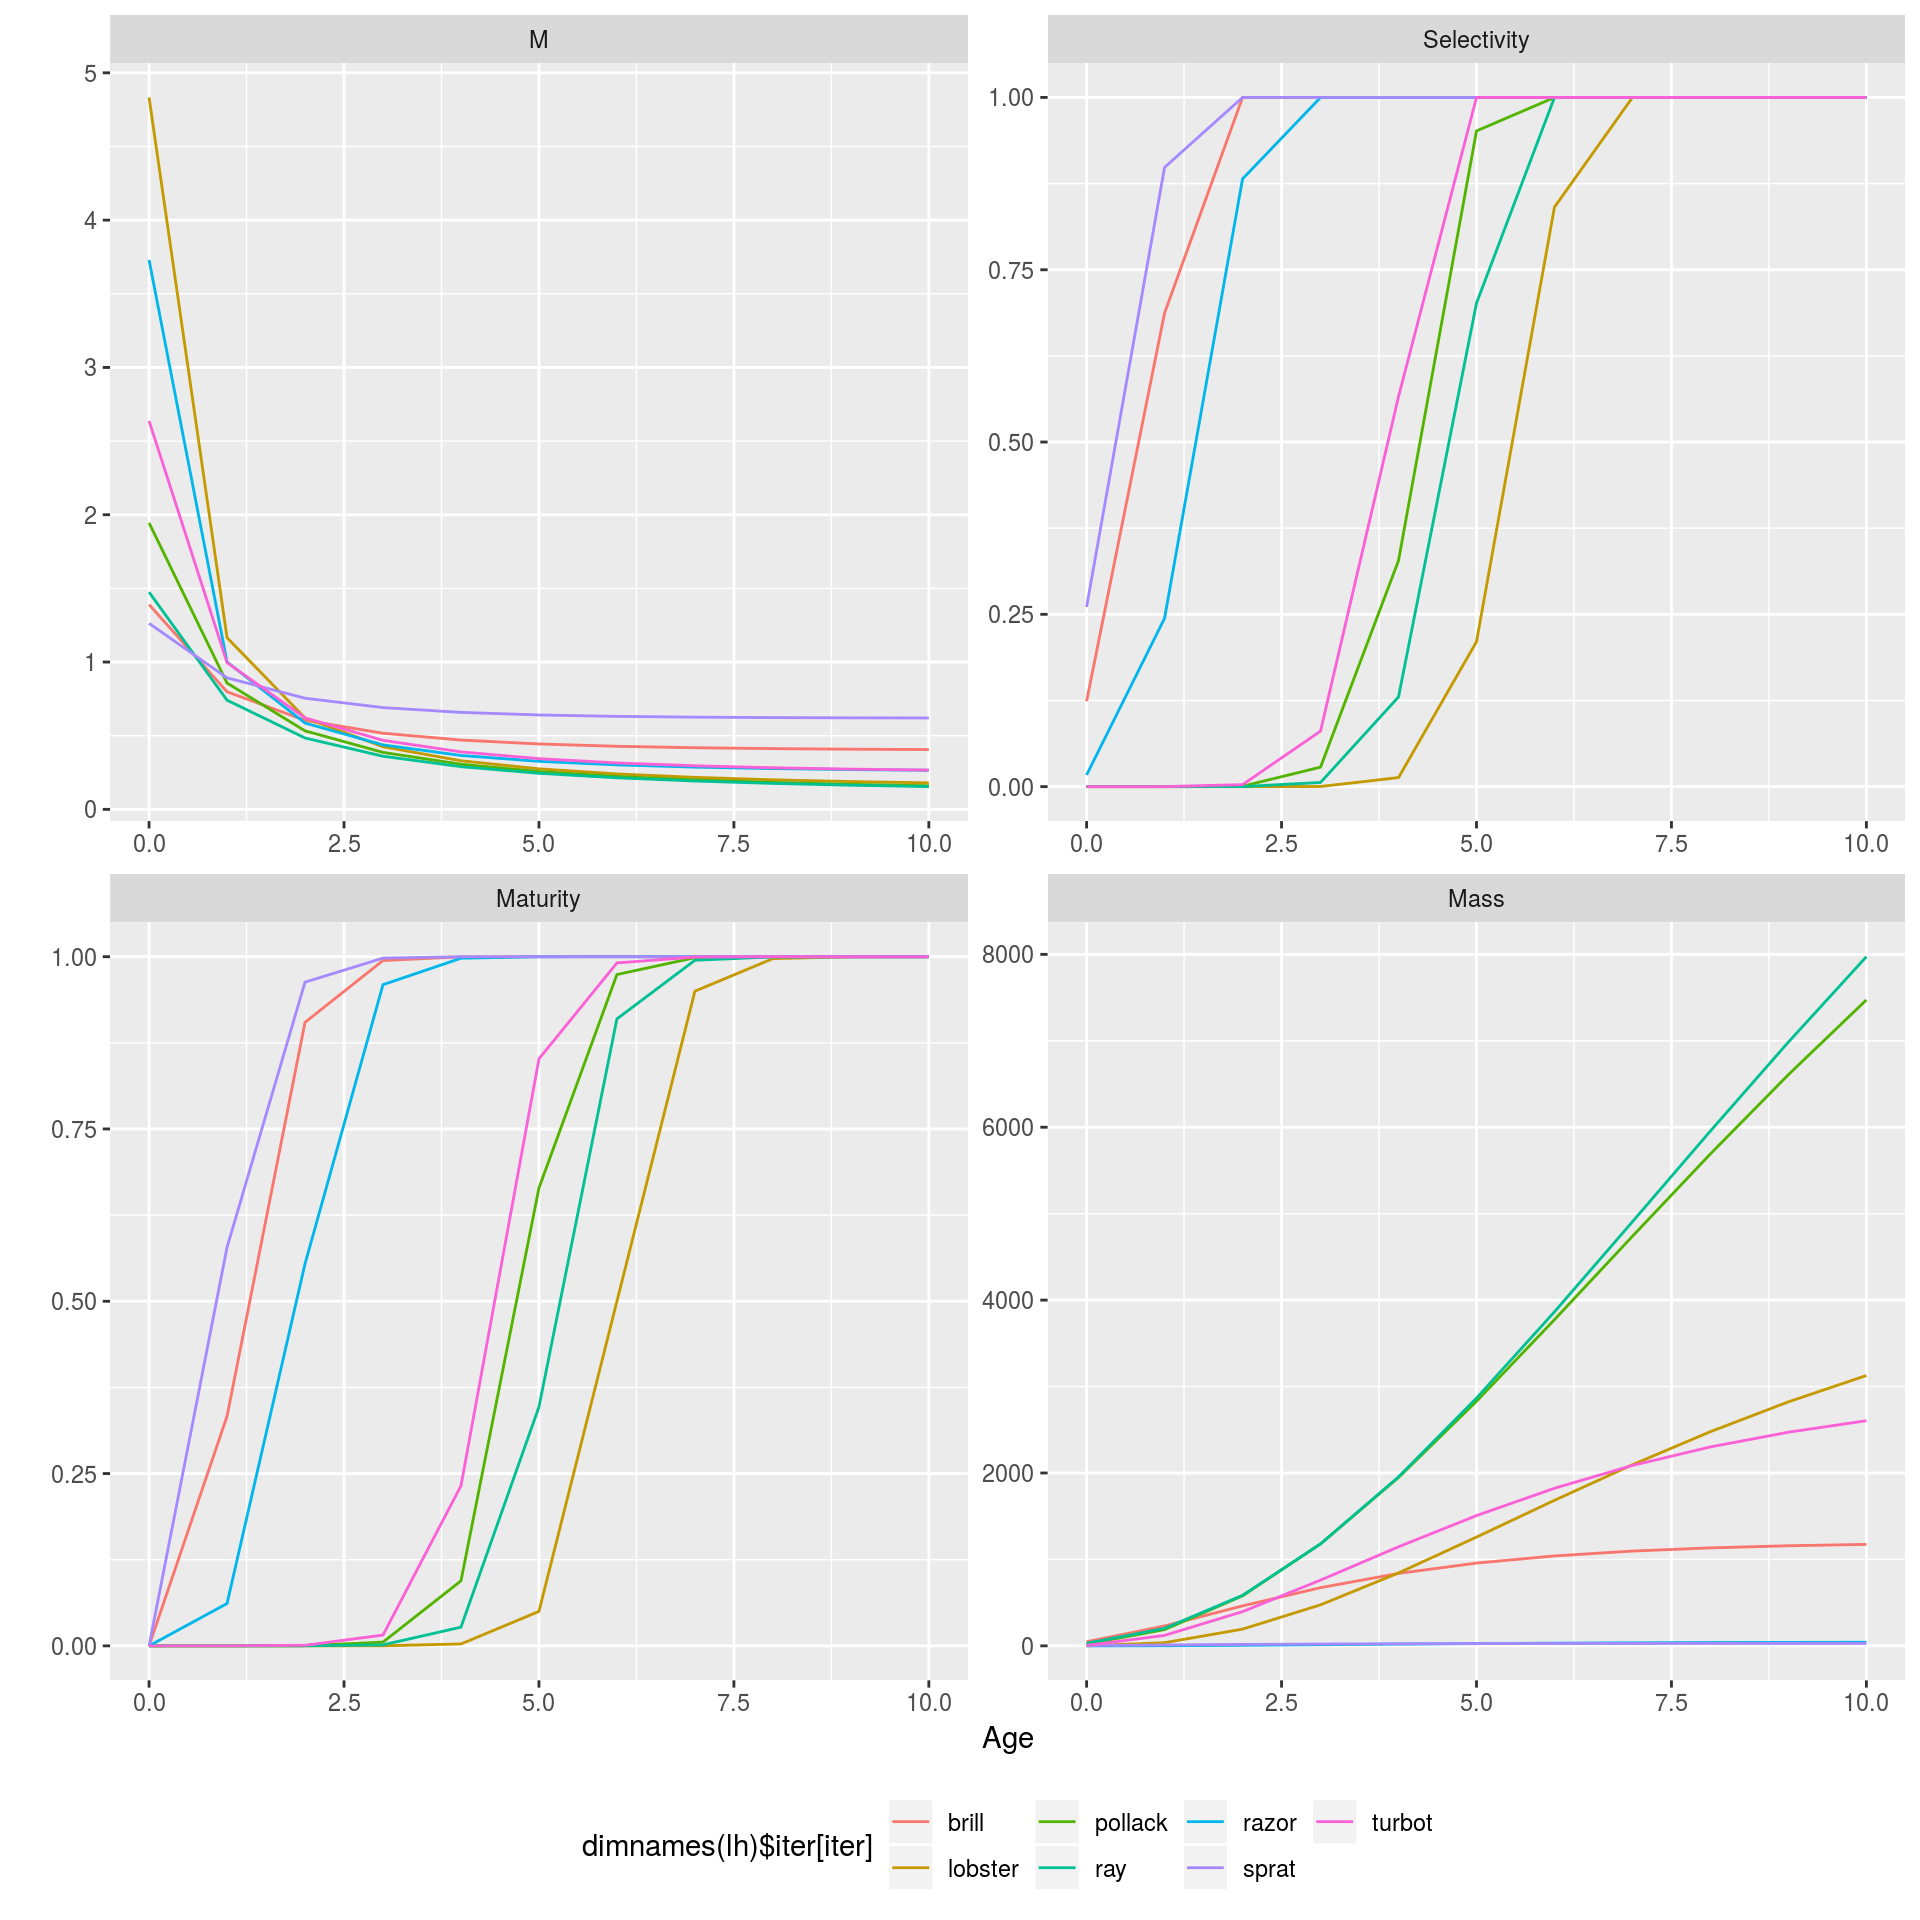
\includegraphics[width=5in]{rg-vectors-1.png}\caption{}\label{fig:vector}\end{figure}
\begin{figure}[]\centering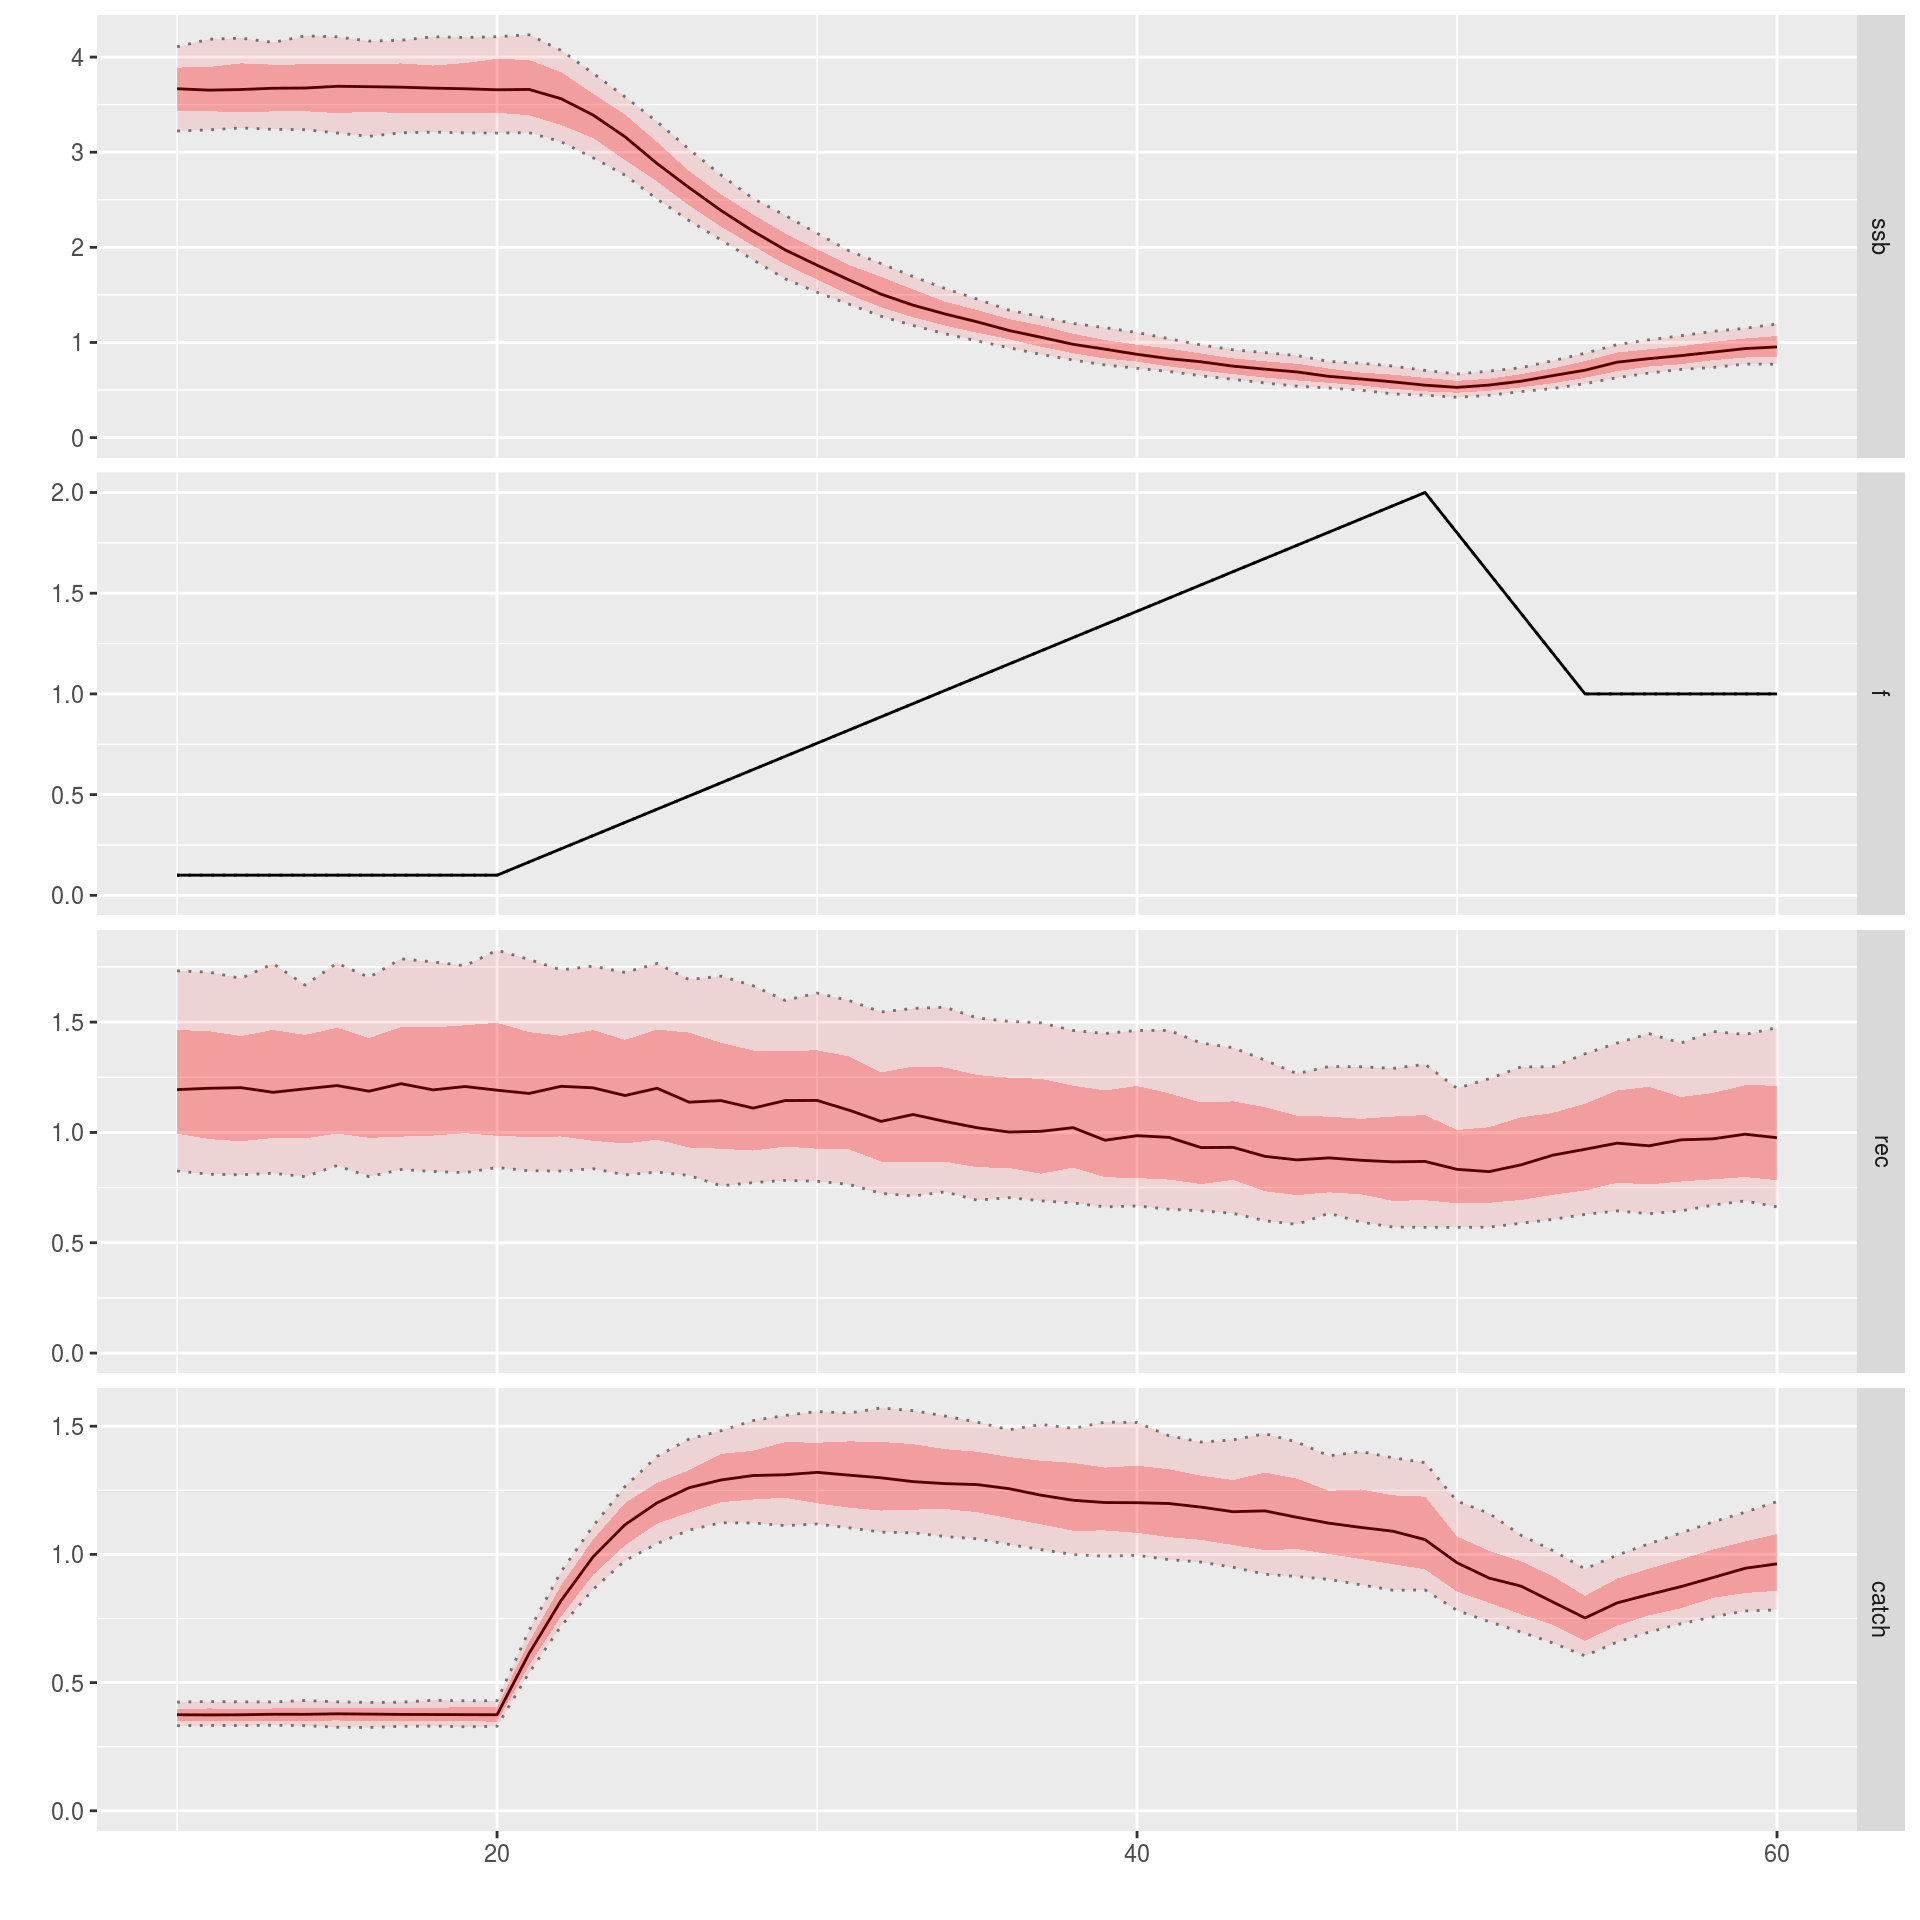
\includegraphics[width=5in]{rg-ts-1.png}\caption{}\label{fig:ts}\end{figure}
\begin{figure}[]\centering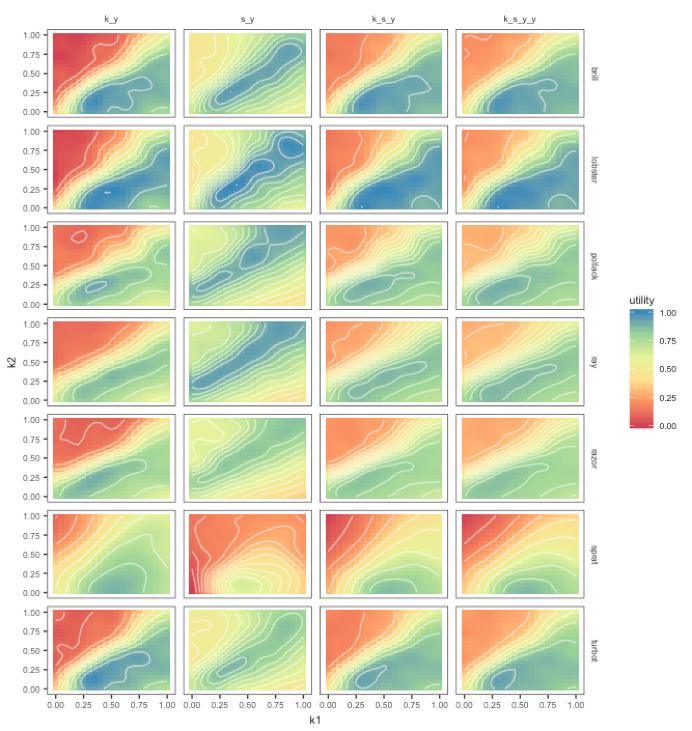
\includegraphics[width=5in]{util.png}\caption{}\label{fig:util}\end{figure}


%% Authors are advised to submit their bibtex database files. They are
%% requested to list a bibtex style file in the manuscript if they do
%% not want to use model1-num-names.bst.

%% References without bibTeX database:

% \begin{thebibliography}{00}

%% \bibitem must have the following form:
%%   \bibitem{key}...
%%

% \bibitem{}

% \end{thebibliography}


\end{document}

%%
%% End of file `elsarticle-template-1-num.tex'.